\providecommand{\main}{../..}

\documentclass[../../thesis]{subfiles}


\begin{document}

\chapter{Kiến thức nền tảng}

Chương này giới thiệu sơ qua về các nền tảng trong quá trình xây dựng ứng dụng.

\begin{itemize}
    \item
        Hai nền tảng đầu tiên liên quan đến nhau, là tiền đề cho toàn bộ ứng
        dụng sẽ được giới thiệu trước, gồm hệ điều hành Android và ngôn ngữ lập
        trình Kotlin.
    \item
        Tiếp theo, lựa chọn về kiến trúc tổng quan, liên quan đến giao diện của
        ứng dụng được trình bày.
    \item
        Sau đó, cơ sở dữ liệu một số phần mở rộng của nó dùng trong ứng dụng sẽ
        được nhắc qua.
    \item
        Cuối cùng là thông tin về CBZ - định dạng tệp tin mà ứng dụng đọc, gồm
        hai phần: sơ lược về định dạng ZIP mà CBZ dựa trên, và các trường
        metadata trong tệp tin CBZ - nguồn thông tin quan trọng để quản lí
        truyện.
\end{itemize}


%----------------------------------------------------------------------------------------
%	2.1: Hệ điều hành Android
%----------------------------------------------------------------------------------------

\section{Hệ điều hành Android}

Android là một hệ điều hành do Google phát triển cho thiết bị di động. Android
dùng nhân Linux và được thiết kế cho màn hình cảm ứng. Cùng với iOS của Apple,
Android trở thành một phần không thể thiếu của cuộc cách mạng di động bắt đầu
vào cuối những năm 2000.

Google mua lại phiên bản Android đầu của công ty khởi nghiệp cùng tên vào năm
2005, và phát triển hệ điều hành này từ đó. Ngoài Google, Android còn nhận đóng
góp lớn từ cộng đồng, do là một dự án mã nguồn mở (phần lớn mã nguồn dùng giấy
phép Apache); tên chính thức của dự án là Android Open Source Project. Dù vậy,
mọi thiết bị Android thương mại đều có ứng dụng độc quyền. Ví dụ đáng kể là bộ
Google Mobile Service, chứa những ứng dụng không thể thiếu như trình duyệt
Chrome hay chợ Play Store. Về mặt này, Android khá giống Chrome: thành phần cốt
lõi kĩ thuật được phát triển theo mô hình mã nguồn mở (AOSP và Chromium), còn
thành phần liên quan đến trải nghiệm người dùng được phát triển riêng.

\begin{wrapfigure}[20]{r}{8.6cm}
    \centering
    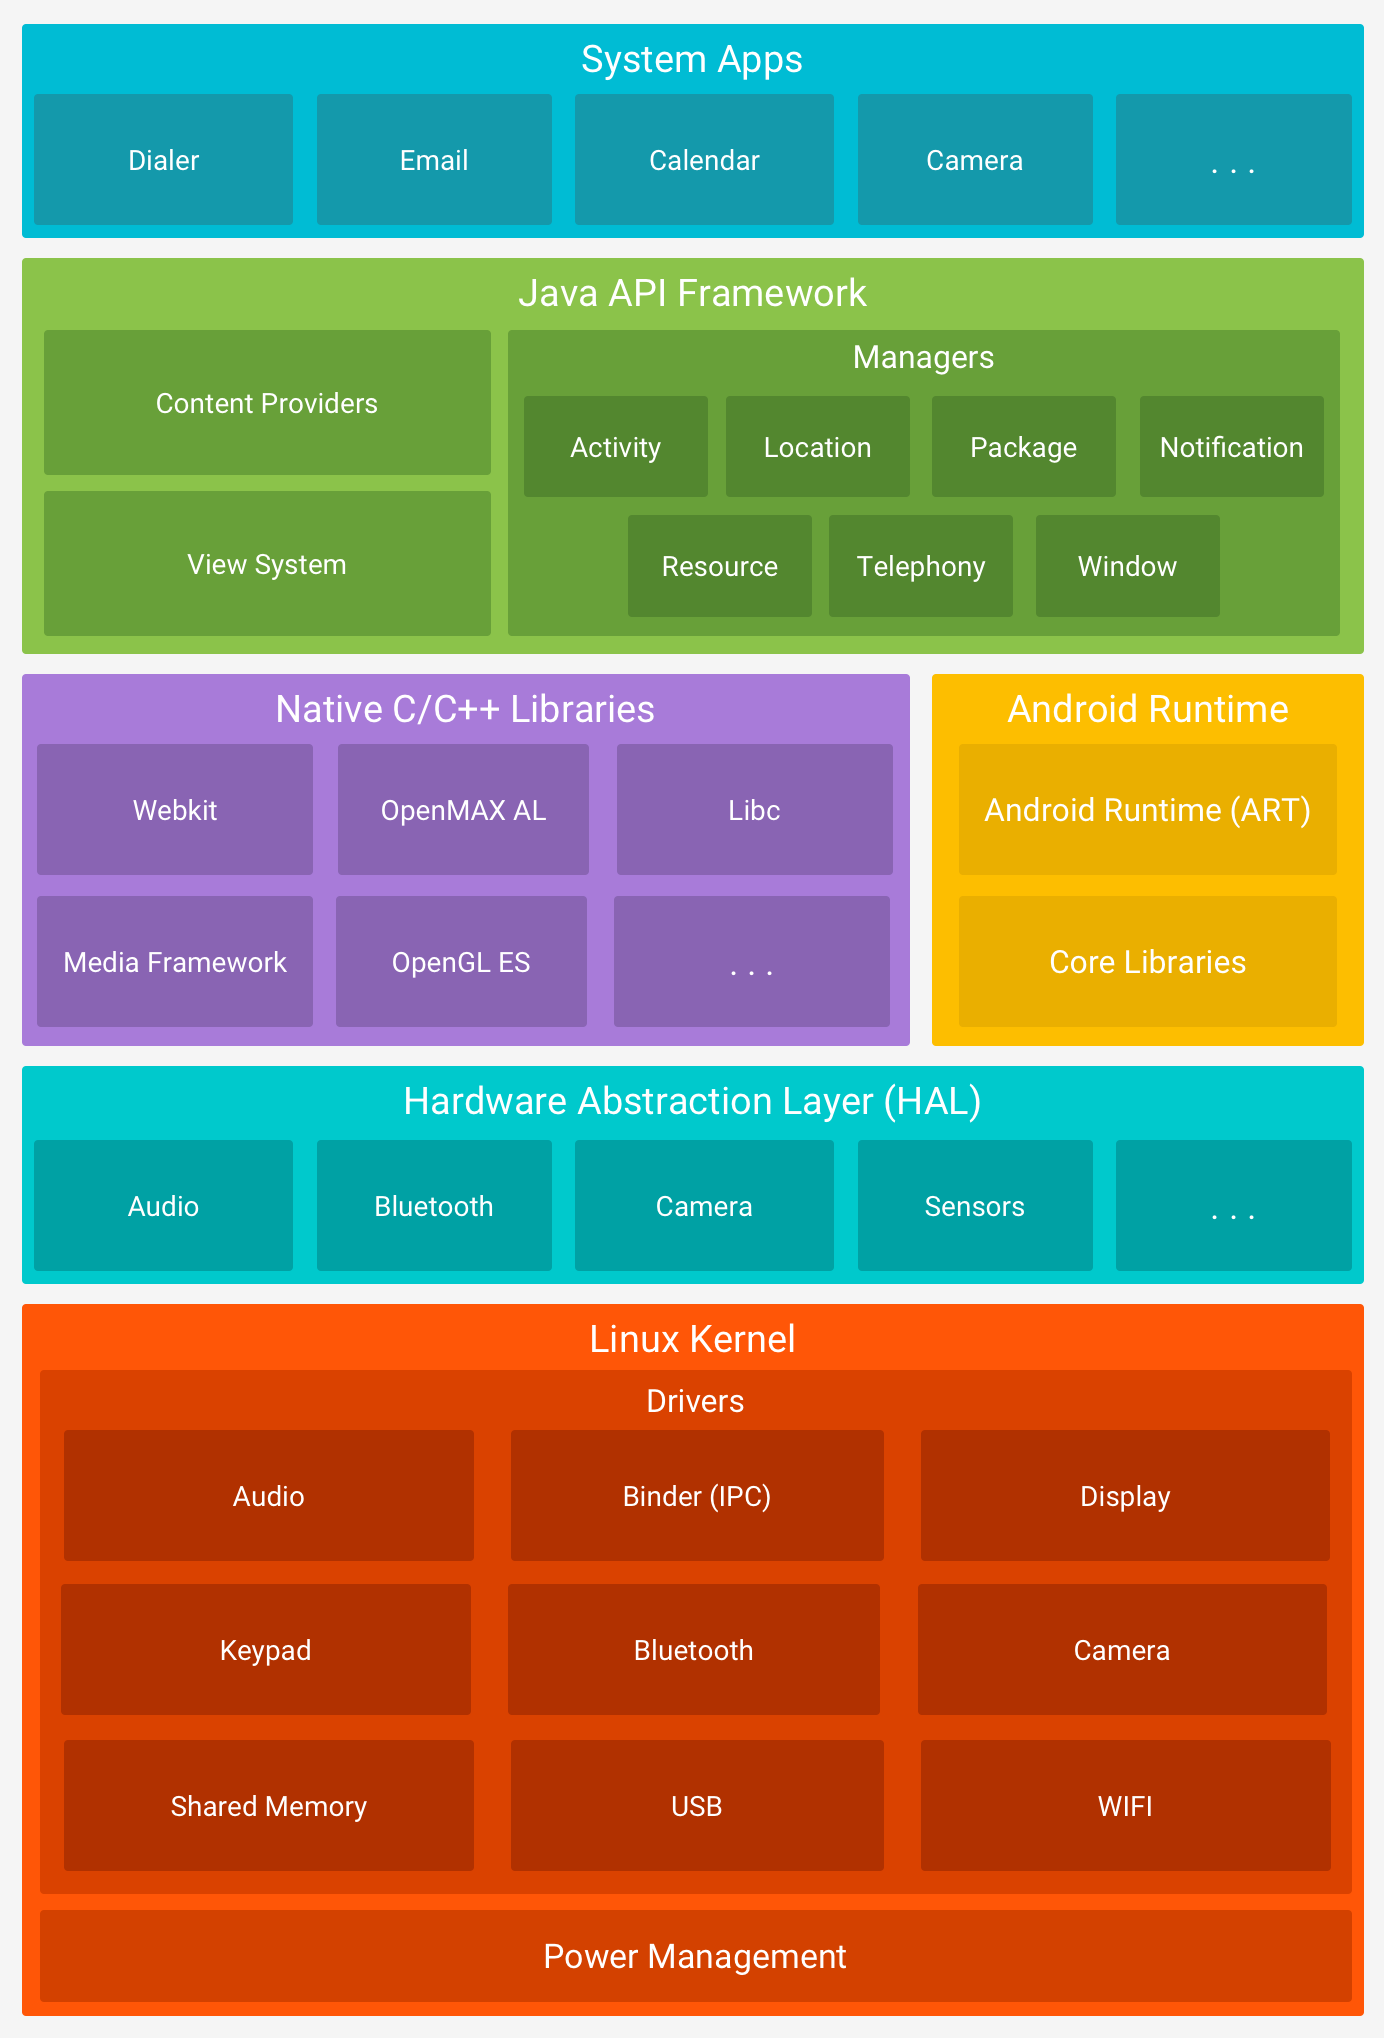
\includegraphics[width=\linewidth]{../images/android-stack_2x.png}
    \vspace*{-10mm}
    \caption{Các phân lớp của Android \cite{GOOGL_ANDR_ARCH}}
    \label{fig:android-stack}
\end{wrapfigure}

Hệ điều hành Android được phân lớp như sau:

\begin{itemize}
    \item
        Nhân Linux (Linux Kernel):

        Đây là tầng thấp nhất. Android dùng nhánh hỗ trợ dài hạn (LTS) của
        Linux. Không như kiểu phát triển distro trên máy tính (chủ yếu thay đổi
        ở ngoài nhân), Google sửa và thêm bớt nhiều thành phần vào nhân trước
        khi tích hợp.
    \item
        Lớp phần cứng trừu tượng (Hardware Abstraction Layer):

        Tầng này trừu tượng hóa các chi tiết phần cứng bằng cách đưa ra các giao
        diện chung cho một kiểu phần cứng nào đó, giúp các tầng trên không cần
        quan tâm đến chi tiết riêng của phần cứng.

    \item
        Android Runtime (ART):

        Ứng dụng Java cần thêm một ứng dụng để chuyển bytecode thành mã máy.
        Trên desktop, đó là các máy ảo Java (JVM). Trên Android, Android Runtime
        nhận nhiệm vụ này. Hai máy ảo này khác nhau ở chỗ ART \emph{biên dịch}
        bytecode thành mã máy (trước khi chạy - AOT), còn JVM \emph{thông dịch}
        bytecode thành mã máy (trong khi chạy).

        ART hiện hỗ trợ đa số tính năng của Java 8.
\end{itemize}

% Split itemize to avoid confusing wrapfigure
% https://tex.stackexchange.com/a/285760/206774
\begin{itemize}[resume, before = \vspace*{-\dimexpr\topsep+\partopsep\relax}]
    \item
        Thư viện C/C++:

        Tầng thư viện native nằm ngang hàng với ART, phục vụ các tiến trình hệ
        thống và một số ứng dụng dùng NDK (tức gọi API C cấp thấp) như trò chơi
        điện tử.
    \item
        Khung phát triển ứng dụng (Java API Framework):

        Mọi ứng dụng Java được viết nhờ sử dụng các thành phần của tầng này
        thông qua API Java. Tầng này cung cấp toàn bộ tính năng của Android cho
        lập trình viên, bao gồm các yếu tố cơ bản như giao diện (View System),
        truy xuất,\ldots

        Lập trình viên có quyền truy cập vào lớp này tương đương với ứng dụng hệ
        thống. Đây có thể coi là một cam kết tránh độc quyền công nghệ, tức đa
        số ứng dụng hệ thống không có khả năng đặc biệt, hay hiệu năng cao hơn
        ứng dụng bên thứ ba tương tự.
    \item
        Ứng dụng hệ thống (System Apps)

        Android đi kèm với một số ứng dụng hệ thống như ứng dụng SMS, trình
        duyệt,\ldots{} Google cho phép thay thế đa số các ứng dụng này với ứng
        dụng bên thứ ba, tuy nhiên có những ngoại lệ như ứng dụng Cài đặt
        (Settings).
\end{itemize}

Gần như mọi ứng dụng Android cơ bản đều sử dụng thành phần View System trong
tầng Khung phát triển để viết giao diện, và yacv không là ngoại lệ. yacv còn sử
dụng thành phần Content Provider, cụ thể là bộ Storage Access Framework, và sẽ
được đề cập ở các phần sau.

\subsection{Android Jetpack}

Jetpack là bộ thư viện giúp viết ứng dụng Android nhanh gọn, ít lỗi hơn so với
việc tự viết những đoạn mã tương tự. Jetpack gồm hai thành phần:

\begin{itemize}
    \item
        AndroidX: đưa \emph{API} của phiên bản hệ điều hành mới lên máy cũ
    \item
        Architecture Component: đưa ra \emph{thư viện} hoàn toàn mới
\end{itemize}

Việc cập nhật Android rất khó khăn do phải chờ nhà sản xuất tối ưu. Do đó,
Google viết AndroidX, trước gọi là Thư viện Hỗ trợ (Support Library), để đưa API
Android mới lên máy cũ. Chú ý rằng Jetpack chỉ có ích cho lập trình viên (API
mới tiện hơn thực ra là wrapper của API sẵn có), chứ không cập nhật tính năng hệ
điều hành.

yacv sử dụng nhiều thành phần của Jetpack, trong đó đáng kể đến ba thư viện sau:

\begin{itemize}
    \item
        LiveData: giúp giao diện luôn được cập nhật theo dữ liệu mới nhất
    \item
        ViewModel: giúp tách dữ liệu và giao diện
    \item
        Room: giúp việc lưu dữ liệu trong SQLite thuận tiện hơn
\end{itemize}

Room là một phần quan trọng của yacv, do đó sẽ được giới thiệu chi tiết ở
\protect\hyperlink{P2.4.2-room}{mục sau}.


%----------------------------------------------------------------------------------------
%	2.2: Ngôn ngữ lập trình Kotlin
%----------------------------------------------------------------------------------------

\section{Ngôn ngữ lập trình Kotlin}

Java là ngôn ngữ lập trình đầu tiên được hỗ trợ trên Android, nhưng không phải
duy nhất. Từ 2019, Google khuyên lập trình viên viết ứng dụng trên Kotlin, một
ngôn ngữ mới do JetBrains phát triển. Giới thiệu lần đầu vào năm 2011, Kotlin
được định hướng trở thành lựa chọn thay thế cho Java. Điều đó thể hiện ở việc
Kotlin tương thích hoàn toàn với Java (từ Java gọi được Kotlin và ngược lại), do
cùng được biên dịch thành JVM bytecode.

Điểm mạnh của Kotlin so với Java là tính ngắn gọn. Do được phát triển mới,
Kotlin không cần tương thích với phiên bản cũ, cho phép dùng các cú pháp hiện
đại, gọn ghẽ. Ngoài ra, vì được một công ty tư nhân phát triển, Kotlin không cần
chờ đến các cuộc họp phức tạp để đạt đồng thuận về tính năng mới, giúp ngôn ngữ
liên tục được cải tiến. Đồng thời, công ty cũng mở mã nguồn của Kotlin và chương
trình dịch, giúp đẩy nhanh quá trình phát triển và tạo thiện cảm cộng đồng cho
một ngôn ngữ non trẻ.

Sau đây là tóm tắt một số đặc điểm kĩ thuật của Kotlin:

\begin{itemize}
    \item
        Về mô hình, Kotlin hỗ trợ hướng đối tượng như Java, nhưng còn có hướng
        hàm, thể hiện ở tính năng hàm ẩn danh (lambda), và hàm được coi là
        first-class.
    \item
        Về hệ thống kiểu, Kotlin giống hệt Java:

        \begin{itemize}
            \item
                Là kiểu tĩnh (statically typed), tức kiểu được kiểm tra khi biên
                dịch (thay vì khi chạy, như Python, JavaScript,\ldots)
            \item
                Là kiểu mạnh (strongly typed), tức không cho phép chuyển kiểu
                ngầm
        \end{itemize}
    \item
        Về cú pháp, Kotlin gọn và hiện đại: bỏ dấu \texttt{;} cuối dòng,
        template literal,\ldots
    \item
        Về lỗi, Kotlin luôn được quảng cáo về khả năng chống
        \texttt{NullPointerException}. Kotlin ``né'' lỗi này do buộc người viết
        đánh dấu cụ thể rằng một đối tượng có thể bị \texttt{null} hay không
        bằng hậu tố \texttt{?} ở khai báo kiểu. Từ đó, Kotlin biết chính xác đối
        tượng có thể là \texttt{null} hay không, và buộc xử lí nếu có.
\end{itemize}

Do Google khuyên dùng Kotlin khi viết ứng dụng Android, tôi cho rằng khóa luận
này là một cơ hội phù hợp để thử Kotlin thay vì dùng Java quen thuộc, và quyết
định chọn viết yacv bằng Kotlin.

\subsection{Coroutine}

\subsubsection{Giới thiệu}

Một thư viện quan trọng của kotlin là \emph{coroutine}. Coroutine giúp viết ứng
dụng có tính tương tranh (concurrency) và bất đồng bộ (asynchronous) một cách
đơn giản hơn.

Về cơ bản, coroutine giống với luồng (thread), nhưng nhẹ hơn. Coroutine luôn
dùng mô hình \emph{đa nhiệm hợp tác} (cooperative multitasking), khác với luồng
hay dùng đa nhiệm ưu tiên (preemptive multitasking). Mấu chốt khác biệt của
chúng là đa nhiệm hợp tác có các ``điểm dừng'' do người viết tạo; khi chạy đến
đó, coroutine có thể dừng lại, chủ động nhả CPU cho việc khác, rồi tiếp tục việc
đang dở vào lúc thích hợp. Ngược lại, đa nhiệm ưu tiên có thể buộc một luồng
đang chạy ngừng lại bất kì lúc nào để ưu tiên chạy một luồng khác. Đây cũng là
điểm khiến coroutine nhẹ hơn: chi phí chuyển ngữ cảnh (context switching) được
kiểm soát và cắt giảm, do chuyển sang thực thi một coroutine khác chưa chắc đã
chuyển sang một luồng hệ điều hành khác.

Với những điều trên, coroutine chưa làm được nhiều. Roman Elizarov, trưởng dự án
Kotlin, hướng coroutine trong Kotlin theo một ý tưởng mới: \emph{tương tranh có
cấu trúc} (structured concurrency, từ đây gọi tắt là SC). Ý tưởng này tiếp tục
đơn giản hóa việc viết những đoạn mã tương tranh bằng cách áp đặt một số giới
hạn, cấu trúc cơ bản. Kết quả là coroutine trong Kotlin hỗ trợ việc xử lí lỗi và
ngừng tác vụ bất đồng bộ tốt hơn việc dùng luồng, hay các thư viện tương tranh
như RxJava.

Coroutine được dùng để tăng tốc những đoạn mã chạy chậm trong yacv (sẽ được mô
tả sau). Ngoài cải thiện về hiệu năng, coroutine và tương tranh có cấu trúc còn
cho phép viết mã ngắn gọn, rõ ràng hơn. Do có tác động lớn, coroutine sẽ được
giới thiệu kĩ hơn ở phần này.

\subsubsection{Bài học từ quá khứ: lập trình có cấu trúc}

\begin{wrapfigure}{r}{5cm}
    \centering
    \vspace*{-6mm}
    \includesvg[width=\linewidth]{../images/sequential-and-go-to-schematic.svg}
    \vspace*{-10mm}    % Manually make figure & caption closer together
    \caption{Lập trình phi cấu trúc với \texttt{GOTO} \cite{NJS_SC}}
    \label{fig:non-structured-programming}
\end{wrapfigure}

Để hiểu về SC, ta có thể so sánh nó với \emph{lập trình có cấu trúc} (structured
programming). Để hiểu sơ về lập trình có cấu trúc, ta phải tìm về \emph{lập
trình phi cấu trúc} (non-structured programming), với đặc điểm là lệnh nhảy
\texttt{GOTO}. Trong buổi đầu của máy tính, lệnh này được dùng nhiều vì hợp với
cách máy tính chạy \cite{NJS_SC}.

Vấn đề của lập trình phi cấu trúc, hay của \texttt{GOTO}, có thể tóm gọn như
sau:

\begin{itemize}
    \item
        Khó nắm bắt luồng chương trình

        Khi đã chạy \texttt{GOTO}, các lệnh phía sau nó không biết khi nào mới
        chạy, vì chương trình chuyển sang lệnh khác mà không trở lại. Luồng chạy
        trở thành một đống ``mì trộn'' như Hình 3, thay vì tuần tự từ trên
        xuống. Tệ hơn, tính trừu tượng bị phá vỡ: khi gọi hàm, thay vì có thể bỏ
        qua chi tiết bên trong, ta phải biết rõ để xem có lệnh nhảy bất ngờ nào
        không.
\end{itemize}

% \begin{wrapfigure}{l}{5cm}
%     \centering
%     \includesvg[width=\linewidth,inkscapelatex=false]
%         {../images/flow-matic-4.svg}
%     \caption{Sự lộn xộn của lập trình phi cấu trúc}
%     \label{fig:goto-spaghetti}
% \end{wrapfigure}

\begin{itemize}[resume, before = \vspace*{-\dimexpr\topsep+\partopsep\relax}]
    \item
        Không cài đặt được các chức năng mới (ngoại lệ, quản lí tài nguyên tự
        động,\ldots)

        Xét ví dụ Java sau về quản lí tài nguyên tự động:

        \begin{minted}{Java}
        try (Scanner scanner = new Scanner(new File("f.txt"))) {
            goto(SOMEWHERE);    // Giả sử Java có GOTO
        }
        \end{minted}

        Do không trả lại luồng điều khiển, việc đóng luồng nhập từ tệp cũng
        không chắc chắn xảy ra, dẫn đến rò rỉ tài nguyên, làm khối lệnh vô dụng.

        Điều gần tương tự cũng khiến việc xử lí ngoại lệ và nhiều tính năng khác
        trở nên rất khó đạt được, một khi ngôn ngữ cho phép \texttt{GOTO}.
\end{itemize}

\begin{wrapfigure}{r}{5cm}
    \centering
    \vspace*{-6mm}
    \includesvg[width=\linewidth]{../images/control-schematics.svg}
    \vspace*{-10mm}
    \caption{Ba cấu trúc cơ bản của lập trình có cấu trúc: rẽ nhánh \texttt{if},
        lặp \texttt{for} và gọi hàm \cite{NJS_SC}}
    \label{fig:3-basic-construct}
\end{wrapfigure}

Lập trình có cấu trúc đơn giản hóa luồng chạy bằng cách giới hạn các lệnh nhảy
còn \texttt{if}, \texttt{for} và gọi hàm. Khác biệt mấu chốt của ba lệnh này so
với \texttt{GOTO} là chúng \emph{trả luồng điều khiển} về điểm gọi, thể hiện rõ
ở \autoref{fig:3-basic-construct}. Theo định nghĩa, ba lệnh trên giải quyết được
hậu quả đầu tiên. Đồng thời, các hậu quả số hai cũng được giải quyết, do ngôn
ngữ đã có cấu trúc (cụ thể là có call stack).

Ngày nay, ba cấu trúc trên đã trở thành phần không thể thiếu trong mọi ngôn ngữ
lập trình, và \texttt{GOTO} chỉ còn dùng trong hợp ngữ. Quá khứ cho thấy nếu áp
dụng một số cấu trúc, giới hạn, ta có thể giải quyết vấn đề một cách tinh tế và
gọn gàng. Trong trường hợp này, SC có thể loại bỏ một số điểm yếu của các API
tương tranh/bất đồng bộ truyền thống, giống cách lập trình có cấu trúc đã làm.

\subsubsection{Áp dụng vào hiện tại: tương tranh có cấu trúc}

Trước hết, ta xem xét hai kiểu API tương tranh hay dùng hiện nay:

% Verbatim can't be put inside macro
% https://tex.stackexchange.com/questions/25190/defining-a-command-for-a-minted-environment#comment49208_25190
% \newcommand{\PythonExample}{
%     \begin{minted}{Python}
%         Thread(target=fn).start() \# Python
%     \end{minted}
% }

\begin{table}[H]
    \centering
    \caption{Hai kiểu API tương tranh hay dùng \cite{NJS_SC}}
    \label{table:2-async-apis}
    \begin{tabular}{r p{4.7cm} l}
        \toprule
        Tên         & Giải thích                                                 & Ví dụ \\
        \midrule
        Tương tranh & Chạy một hàm theo cách tương tranh với luồng chạy hiện tại & \mintinline{python}{Thread(target=fn).start() \# Python} \\
        Bất đồng bộ & Chạy một hàm khi có sự kiện xảy ra (callback)              & \mintinline{js}{element.onclick = cb; // JS} \\
        \bottomrule
    \end{tabular}
\end{table}

\begin{wrapfigure}[5]{r}{5cm}
    \centering
    \includesvg[width=\linewidth]{../images/sequential-and-go-to-schematic.svg}
    \vspace*{-10mm}
    \caption{Tương tranh phi cấu trúc với \texttt{goroutine} - API kiểu tương
        tranh \cite{NJS_SC}}
    \label{fig:goroutine}
\end{wrapfigure}

Qua \autoref{fig:goroutine}, không khó để thấy rằng mọi vấn đề của lập trình phi
cấu trúc đều lặp lại với hai API trên:

\begin{itemize}
    \item
        Ta xem lại ví dụ quản lí tài nguyên tự động. Nếu có luồng thực thi khác
        tương tranh với luồng chính, thì khi luồng chính đóng \texttt{Scanner},
        có thể luồng kia đang đọc dở. Do đó, tính năng này không thể hoạt động.
\end{itemize}

\begin{itemize}[resume, before = \vspace*{-\dimexpr\topsep+\partopsep\relax}]
    \item
        Với tính năng bắt ngoại lệ, nếu có ngoại lệ ở luồng tương tranh, ta cũng
        không có cách nào để biết, và buộc phải kệ nó.
\end{itemize}

Trên thực tế, có cách để thực hiện một số chức năng trên với API hiện tại, tuy
vậy đó đều là cách xử lí riêng, do đó chưa thực sự thuận tiện khi dùng. Ví dụ,
ES6 có \texttt{catch()} để bắt ngoại lệ trong \texttt{Promise} mà không (thể)
dùng cấu trúc \texttt{try-catch} sẵn có. Với SC, các vấn đề này đều được giải
quyết.

Trong \autoref{fig:kotlin-coroutine}, ta xét một đoạn mã tương tranh dùng
coroutine trong Kotlin, tức dùng SC (không phải coroutine trong mọi ngôn ngữ đều
dùng mô hình này).

\begin{wrapfigure}{l}{8cm}
    \centering
    \vspace*{-4mm}
    \includesvg[width=\linewidth,inkscapelatex=false]    % To leave text as is
        {../images/kotlin-coroutine.svg}                 % https://tex.stackexchange.com/a/595916/206774
    \vspace*{-10mm}
    \caption{Tương tranh có cấu trúc dùng coroutine trong Kotlin \cite{NJS_SC}}
    \label{fig:kotlin-coroutine}
\end{wrapfigure}

Nguyên tắc của SC là: \emph{coroutine cha chờ mọi coroutine con chạy xong}, kể
cả khi nó xong trước. Nguyên tắc này đảm bảo rằng khi một hàm kết thúc, không
còn tác vụ tương tranh nữa, và luồng điều khiển hợp nhất được trả về điểm gọi.
Đột nhiên, hai tính năng có vấn đề ở trên lại hoạt động:

\begin{itemize}
    \item
        Quản lí tài nguyên tự động: do đảm bảo trả lại luồng điều khiển, tài
        nguyên đảm bảo được đóng; do không còn tác vụ con, tài nguyên không bị
        đọc sau đóng.
\end{itemize}

\begin{itemize}[resume, before = \vspace*{-\dimexpr\topsep+\partopsep\relax}]
    \item
        Bắt ngoại lệ: do cấu trúc cha-con (khác với các API hiện tại cho rằng
        hai tác vụ tương tranh là ngang hàng), coroutine con có thể ném ngoại lệ
        để coroutine cha bắt.
\end{itemize}

Chú ý là các API hiện tại không phải không làm được nguyên tắc trên, vấn đề là
thực hiện một cách \emph{tự động} và \emph{đảm bảo}. Ví dụ, trong JS, để tuân
theo nguyên tắc này, ta cần \texttt{await} với mọi hàm \texttt{async}; nếu
không, luồng chạy của hàm đó sẽ tách biệt với luồng chương trình, như Hình 5 mô
tả. Do không có ràng buộc chặt chẽ kia, các tính năng ngôn ngữ mới cũng khó cài
đặt như đã phân tích.

Do trong các ngôn ngữ khác, nguyên tắc trên chỉ là một ca sử dụng, việc ép buộc
viết theo ca sử dụng này đòi hỏi lập trình viên thay đổi suy nghĩ về mã tương
tranh. Đổi lại, chương trình trở nên sáng rõ, giống với những đoạn mã viết theo
kiểu tuần tự truyền thống.

Một khi vấn đề tương tranh được giải quyết hoặc đơn giản hóa, việc song song hóa
(paralellization) để tăng tốc ứng dụng chỉ còn là một chi tiết cài đặt.

\subsubsection{Tóm tắt}

Coroutine với SC là một trong những tính năng quan trọng nhất của Kotlin, và
được dùng để tăng tốc những đoạn mã chạy chậm trong yacv. Mấu chốt của SC được
tóm gọn trong Hình 6. Dù khá mới (Martin Sústrik, tác giả của ZeroMQ, đưa ra ý
tưởng này năm 2016) và còn tranh cãi, mô hình này vẫn được cải thiện liên tục,
có thư viện ở nhiều ngôn ngữ như Java (Loom), Python (Trio),\ldots{} Điều này
cho thấy ý tưởng có tiềm năng lớn, giúp đơn giản hóa tư duy về tương tranh.


%----------------------------------------------------------------------------------------
%	2.3: Mẫu thiết kế MVVM và Kiến trúc Google khuyên dùng
%----------------------------------------------------------------------------------------

\section{Mẫu thiết kế MVVM và Kiến trúc Google khuyên dùng}

\subsection{Mẫu thiết kế MVVM}

Cũng như các tác vụ lập trình khác, lập trình giao diện sử dụng nguyên lý
Separation of Concern, hiểu đơn giản là chia tách chức năng. Nhiều năm kinh
nghiệm cho thấy giao diện nên được chia làm hai phần chính tách biệt nhau:

\begin{itemize}
    \item
        Model: dữ liệu để hiển thị (trả lời câu hỏi ``cái gì''); liên quan đến
        đối tượng, mảng,\ldots
    \item
        View: cách để hiển thị dữ liệu đó (trả lời câu hỏi ``như thế nào'');
        liên quan đến các yếu tố giao diện như nút, danh sách,\ldots
\end{itemize}

Sự tách biệt thể hiện ở chỗ Model không được biết View. Khi này, giao diện và
nghiệp vụ có thể phát triển khá độc lập với nhau, giúp giảm thời gian phát
triển. Ngược lại, View có thể biết đến Model hay không là tùy vào cách triển
khai cụ thể. Có sự bất đối xứng này là do View thường có các mã liên quan chặt
chẽ đến framework vốn phức tạp để kiểm thử, còn Model thường có các mã đơn giản.

Khó khăn ở đây là làm sao để kết nối hai thành phần riêng biệt kia. Nhiều mô
hình cố giải quyết vấn đề này, tiêu biểu là MVC, MVP và MVVM. Ta lần lượt xem
xét chúng để thấy rằng MVVM phù hợp nhất với Android, do đó được chọn làm nền
tảng cho Kiến trúc Google khuyên dùng.

\subsubsection{MVC: Model - View - Controller}

Phương hướng đầu tiên được thử là MVC, vốn phổ biến vào thời điểm Android ra
đời. Do được phát minh từ lâu và mỗi framework lại có cách giải thích khác nhau,
nên không có một mô hình cụ thể về cách ba thành phần trên tương tác. Tuy vậy,
vẫn có vài điểm chung không đổi:

\begin{enumerate}
    \item
        Controller nhận thao tác người dùng
    \item
        Sau đó, controller cập nhật Model và View
\end{enumerate}

Ngay ở đây, ta đã thấy điểm yếu của MVC khi áp dụng vào Android. Trong Android,
ứng dụng sử dụng Activity và Fragment để viết giao diện. Hai đối tượng này cũng
kiêm luôn việc nhận thao tác người dùng, tức chúng là \emph{cả View và
Controller}. Mục đích tách ra ba đối tượng do đó không thể làm được.

Hiện nay, MVC trên Android được coi là lỗi thời, không phù hợp.

\subsubsection{MVP: Model - View - Presenter}

Năm 2012, Robert Martin ``Uncle Bob'' xuất bản một bài viết nổi tiếng về
kiến trúc phần mềm: Clean Architecture, tạo ra một trào lưu đưa Clean
Architecture đi khắp nơi. MVP, vốn được phát triển từ lâu, được đông đảo
lập trình viên chọn để triển khai Clean Architecture trên Android. Trước
khi Google chọn MVVM, đây là hướng đi mới, có kì vọng cao sau nhiều thất
bại trong việc đưa MVC vào Android.

\begin{wrapfigure}[8]{r}{7cm}
    \centering
    \vspace*{-5mm}
    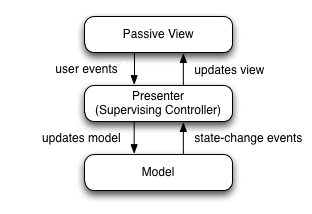
\includegraphics[width=\linewidth]{../images/Model_View_Presenter_GUI_Design_Pattern.png}
    \vspace*{-10mm}
    \caption{Kiến trúc MVP \cite{WIKI_MVP}}
    \label{fig:mvp}
\end{wrapfigure}

Nhiệm vụ của ba thành phần như sau:

\begin{itemize}
    \item
        Model: vẫn như trong MVC
    \item
        View: hiển thị dữ liệu; nhận tương tác người dùng để chuyển sang
        Presenter
    \item
        Presenter: trung gian giữa Model và View: nhận tương tác từ View,
        gọi/thay đổi Model, cập nhật View
\end{itemize}

Ở đây, ta thấy điểm yếu View-Controller nhập nhằng của MVC được khắc phục, khi
View kiêm luôn việc nhận tương tác. Đồng thời, Model và View hoàn toàn không
biết nhau, đúng theo nguyên lý tách lớp của Clean Architecture.

Ta xét một ứng dụng ToDo đơn giản, trong đó các công việc có thể được đánh dấu
đã hoàn thành. Trong ứng dụng, màn hình hiển thị số việc đã và chưa hoàn thành.
Trong màn hình đó, tương tác của MVP như sau:

\begin{enumerate}
    \item
        Presenter lấy tất cả công việc trong Model
    \item
        Presenter đếm số việc hoàn thành, chưa hoàn thành
    \item
        Presenter gọi hàm của View, truyền hai số đếm được ở trên vào
\end{enumerate}

Đến đây, thiết kế đã khá hoàn chỉnh và phù hợp với Android.

\subsubsection{MVVM: Model - View - View Model}

\begin{wrapfigure}{r}{11.5cm}
    \centering
    \vspace*{-6mm}
    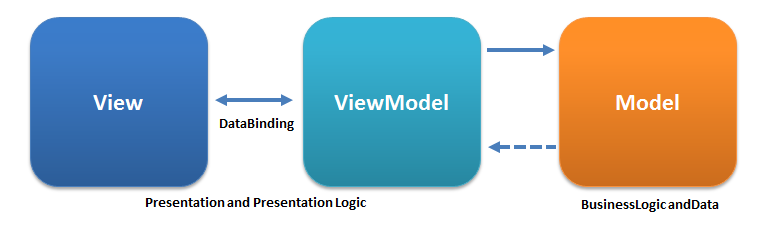
\includegraphics[width=\linewidth]{../images/MVVMPattern.png}
    \vspace*{-10mm}
    \caption{Kiến trúc MVVM \cite{MUN_MVVM}}
    \label{fig:mvvm}
\end{wrapfigure}

Ta quay về chủ đề chính: MVVM. MVVM giống MVP ở chỗ View Model (từ đây gọi tắt
là VM) kết nối View và Model như Presenter. Điểm khác biệt là cách truyền dữ
liệu \cite{MUN_MVVM}:

\begin{itemize}
    \item
          Trong MVP, Presenter gọi hàm của View để truyền dữ liệu cho View
\end{itemize}

\begin{itemize}[resume, before = \vspace*{-\dimexpr\topsep+\partopsep\relax}]
    \item
          Trong MVVM, VM dùng \emph{data binding} để truyền dữ liệu cho View
\end{itemize}

Data binding là cơ chế để \emph{tự động} đưa dữ liệu vào thành phần hiển thị.
Quay lại ví dụ ToDo ở trên, nếu dùng data binding để ``gắn'' (bind) danh sách
công việc vào View, thì khi danh sách thay đổi, View cũng tự động thay đổi theo.

Do dùng data binding thay vì gọi hàm thủ công, VM không cần có tham chiếu tới
View, khác với Presenter. Điều này giúp liên kết View - VM thêm \emph{lỏng lẻo}
(loose coupling), giúp kiểm thử dễ dàng hơn. Phần còn lại của hai mô hình giống
nhau: View cần biết VM để chuyển tương tác; VM cần biết Model để lấy dữ liệu.

Do là mô hình phù hợp nhất trong cả ba với riêng Android, MVVM được chọn làm nền
tảng cho Kiến trúc Google khuyên dùng.

\subsection{Kiến trúc Google khuyên dùng}

Kiến trúc Google khuyên dùng có gốc là mô hình MVVM, có dạng như sau:

\begin{itemize}
    \item
        Repository là Model trong MVVM, giúp VM lấy dữ liệu mà không cần quan
        tâm dữ liệu lấy từ đâu: cơ sở dữ liệu, gọi API qua mạng,\ldots
    \item
        LiveData là cơ chế data binding dùng luồng dữ liệu (stream)
    \item
        Activity/Fragment là View
\end{itemize}

\begin{wrapfigure}{r}{8cm}
    \centering
    \vspace*{-6mm}
    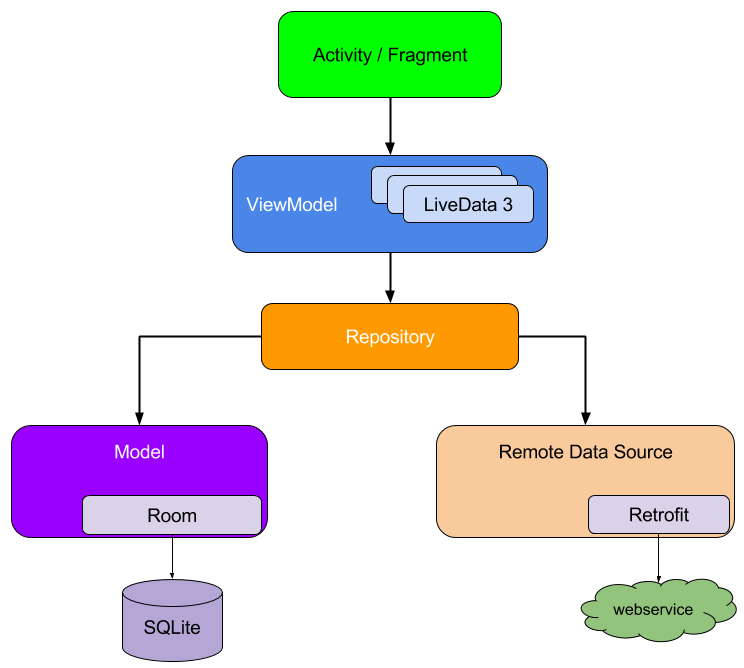
\includegraphics[width=\linewidth]{../images/final-architecture.png}
    \vspace*{-10mm}
    \caption{Kiến trúc Google khuyên dùng \cite{GOOGL_APP_ARCH}}
    \label{fig:google-recom-arch}
\end{wrapfigure}

Repository là một điểm được chi tiết hóa so với MVVM. Google cho rằng một ứng
dụng không nên hoàn toàn vô dụng nếu không có mạng. Do đó, cần có hai nguồn dữ
liệu: dữ liệu từ máy chủ, và dữ liệu đệm, ngoại tuyến. Khi có nhiều nguồn dữ
liệu, mẫu thiết kế Repository là lựa chọn hiển nhiên để trừu tượng hóa chúng.

yacv sử dụng kiến trúc này, dù không có tính năng liên quan đến mạng. Lý do là
yacv có tính năng quét truyện hoạt động chậm giống như giao tiếp mạng, nên cần
dữ liệu đệm và dữ liệu quét thực tế.


%----------------------------------------------------------------------------------------
%	2.4: Cơ sở dữ liệu SQLite
%----------------------------------------------------------------------------------------

\section{Cơ sở dữ liệu SQLite}

SQLite là một hệ quản trị cơ sở dữ liệu quan hệ (RDBMS). Từ ``Lite'' trong tên
có nghĩa là ``nhỏ'', thể hiện mục tiêu thiết kế chính của nó là nhỏ gọn. SQLite
có thể được nhúng vào phần mềm khác ở dạng thư viện, thay vì là một phần mềm
riêng với cấu trúc chủ-khách như MySQL,\ldots{} Ngay từ những phiên bản đầu,
Android đã tích hợp SQLite, giúp lập trình viên không phải nhúng SQLite vào từng
ứng dụng.

Để đạt mục tiêu, SQLite chỉ giữ các tính năng SQL cốt lõi (tạo/đọc/sửa/xóa),
giao dịch (có ACID), và chỉ tối ưu cho việc truy cập từ một ứng dụng cùng lúc.
Các tính năng thường có trong RDBMS cho máy chủ, như nhân bản (replication),
chia dữ liệu tự động (sharding), khóa dòng, đọc ghi nhiều luồng cùng
lúc,\ldots{} được loại bỏ. Do đó, với nhu cầu lưu trữ đơn giản, SQLite vừa nhanh
vừa gọn.

yacv dùng SQLite để lưu đệm thông tin truyện, tránh quét nhiều lần.

\subsection{Thư viện ORM Room}

Room là một thư viện thuộc Jetpack, giúp lập trình viên dùng SQLite tốt hơn. Đây
có thể xem là một thư viện ORM đơn giản cho SQLite. Room tự động làm nhiều công
việc liên quan đến SQL:

\begin{itemize}
    \item
        Tạo bảng: Lập trình viên chỉ cần khai báo các đối tượng dữ liệu như một
        lớp hướng đối tượng thông thường, rồi đánh dấu với Annotation và
        interface của Room. Sau đó, Room sinh các bảng tương ứng.
    \item
        Truy vấn: Lập trình viên chỉ cần viết lệnh SQL. Sau đó, Room sinh hàm
        truy vấn tương ứng, chuyển dữ liệu dạng đối tượng sang dạng để lưu trong
        bảng và ngược lại.
    \item
        Kiểm tra truy vấn khi biên dịch: lỗi lệnh SQL có thể được dò ra ngay khi
        biên dịch chứ không cần chờ đến khi chạy.
    \item
        Kiểm soát lược đồ (schema): Khi thêm/sửa/xóa bảng/cột, Room luôn phát
        hiện và ép lập trình viên viết cơ chế cập nhật. Do đó, ứng dụng dùng
        lược đồ cũ khi được cập nhật sẽ biết cách sửa cơ sở dữ liệu đến phiên
        bản lược đồ mới.
    \item
        Tương thích với LiveData: Room cho phép View cập nhật dữ liệu theo cơ sở
        dữ liệu chỉ bằng vài dòng mã dùng LiveData.
\end{itemize}

\subsection{Tìm kiếm văn bản}

Tìm kiếm văn bản (full-text search, hay gọi tắt là FTS) là một trong số ít các
tính năng nâng cao được giữ lại trong SQLite. Cũng như các thư viện tìm kiếm
khác, SQLite cài đặt chức năng này bằng chỉ mục đảo (inverted index):

\begin{enumerate}
    \item
        Khi dữ liệu văn bản được ghi, nó được tách thành các từ.
    \item
        Các từ được đưa vào từ điển, với khóa là chính từ đó, còn giá trị là ID
        của hàng \texttt{rowid}.
\end{enumerate}

FTS khác với đánh chỉ mục thường (cũng là chỉ mục đảo nhưng cho kiểu dữ liệu
thông thường) ở bước 1: \emph{từng từ} được tách ra, còn chỉ mục thường dùng
\emph{cả} văn bản. Do đó, khi tìm từ lẻ, FTS có thể tìm các hàng chứa từ đó rất
nhanh. Điểm yếu là ghi chậm, kích cỡ lớn hơn chỉ mục thường. Nếu bản thân dữ
liệu văn bản trong cột là một khối, ví dụ như email, chỉ mục thường đã đủ tốt,
không cần FTS.

Trong SQLite, một số kĩ thuật xử lí ngôn ngữ tự nhiên cơ bản cũng được áp dụng
trong bước 1, như rút gọn từ (stemming, dùng thuật toán Porter, ví dụ khi tìm
``run'' sẽ ra được cả ``runs'', ``running'', ``ran''; tất nhiên chỉ đúng với
tiếng Anh), giúp kết quả tìm kiếm linh động hơn.

yacv có tính năng tìm kiếm liên quan đến tiêu đề, tên nhân vật,\ldots{} đều là
những câu văn, đoạn văn. Do đó, FTS có vai trò không thể thiếu để tăng tốc tìm
kiếm trong ứng dụng.


%----------------------------------------------------------------------------------------
%	2.4: Định dạng tệp nén ZIP và CBZ
%----------------------------------------------------------------------------------------

\section{Định dạng tệp nén ZIP và CBZ}

Các tệp truyện mà yacv đọc có định dạng CBZ, về bản chất chính là tệp nén ZIP
thông thường. Do yêu cầu của các phần sau, định dạng tệp ZIP cũng cần được trình
bày ở mức cơ bản.

\subsection{Định dạng tệp nén ZIP}

ZIP là một định dạng tệp nén không mất mát (lossless). Được phát minh vào năm
1989 bởi Phil Katz, ZIP đã trở thành định dạng nén tiêu chuẩn, được hỗ trợ trên
gần như mọi nền tảng, bao gồm Android.

ZIP thực chất là một định dạng chứa (container), chuyên chứa dữ liệu nén, chứ
không phải thuật toán nén; thuật toán nén hay dùng nhất trong ZIP là DEFLATE.
Một trong các mục tiêu của ZIP là giúp việc sửa tệp nén (thêm, sửa, xóa tệp con
trong tệp ZIP) nhanh nhất có thể. Mục tiêu đó thể hiện ở thiết kế sau
\cite{PKWARE_APPNOTE}:

\begin{itemize}
    \item
        Thuật toán nén mỗi tệp gốc thành một tệp nhị phân, ở đây gọi là
        \emph{tệp nén lẻ} (data trong Hình 10). Sau đó, các tệp nén lẻ này được
        nối thành tệp ZIP cuối cùng.
    \item
        Trước mỗi tệp nén lẻ là một header gọi là \emph{File Entry} để lưu thông
        tin liên quan.
    \item
        Ở \emph{cuối} tệp ZIP, sau khi đã nối các tệp nén lẻ và header lại, các
        header được gom lại, lưu một lần nữa vào một cấu trúc gọi là
        \emph{Central Directory}. Có thể so sánh File Entry như các \emph{đề
        mục}, còn Central Directory là \emph{mục lục}.
    \item
        Hai thông tin quan trọng trong File Entry là tên tệp gốc và \emph{vị trí
        bắt đầu} (offset), tức số byte tính từ đầu tệp ZIP đến tệp nén lẻ tương
        ứng.
\end{itemize}

\begin{figure}[H]
    \centering
    % \includesvg[width=10cm,inkscapelatex=false]
    %     {../images/ZIP-64_Internal_Layout.svg}
    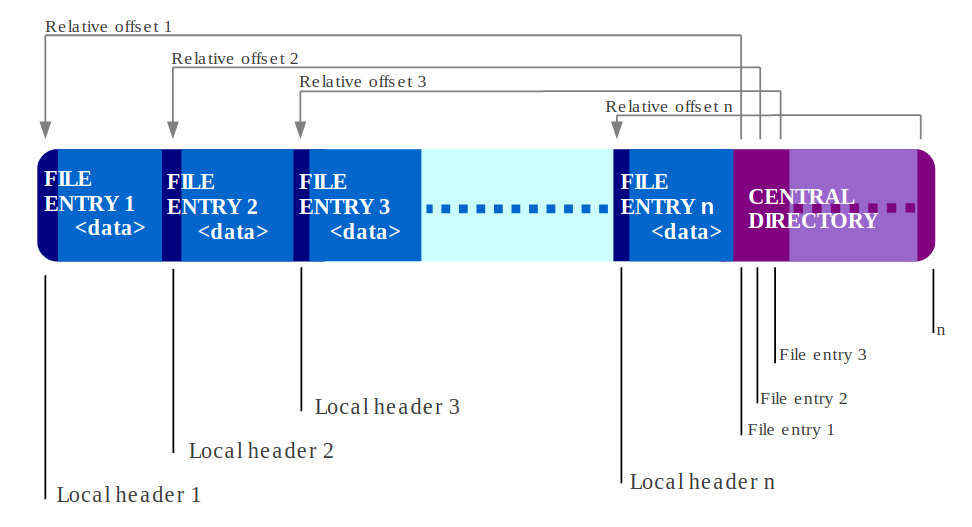
\includegraphics[width=10cm]
        {../images/ZIP-64_Internal_Layout.png}
    \caption{Cấu trúc tệp nén ZIP \cite{WIKI_ZIP}}
    \label{fig:zip_layout}
\end{figure}

Ta phân tích kĩ hơn:

\begin{itemize}
    \item
        Do từng tệp được nén riêng, có thể dùng thuật toán khác nhau cho hiệu
        quả tốt với từng tệp.
    \item
        Cũng do nén riêng, việc thêm/sửa/xóa (gọi chung là sửa) và giải nén có
        thể được thực hiện với từng tệp nén lẻ, thay vì phải giải nén, sửa, rồi
        nén lại toàn bộ.
    \item
        Nhờ mục lục (chứa vị trí tệp nén lẻ), việc sửa còn diễn ra nhanh do ứng
        dụng biết vị trí để đọc ghi dữ liệu.
    \item
        Mục lục đặt ở cuối là tối ưu:

        \begin{itemize}
            \item
                Giả sử mục lục đặt ở đầu. Khi sửa, toàn bộ các tệp nén lẻ phải
                di chuyển để tạo chỗ cho mục lục mới (giống như thêm một phần tử
                vào mảng ở vị trí đầu: toàn bộ các phần tử sau bị đẩy lên để tạo
                chỗ trống).
            \item
                Do mục lục nằm ở cuối tệp tin, khi sửa tệp nén, chỉ cần đẩy các
                tệp nén lẻ từ chỗ sửa. Đây có thể coi là một tối ưu nhỏ, nhưng
                trước đây là một điểm sáng. Do đĩa mềm - phương tiện chia sẻ chủ
                yếu thời đó - có dung lượng nhỏ, tệp ZIP có thể phải cắt ra cho
                vừa. Cách sửa tệp linh động này cho phép chỉ ghi lại dữ liệu ở
                một số đĩa mềm, thay vì ghi lại toàn bộ.
            \item
                Hơn nữa, nếu mục lục ở đầu thì ngay trong khi nén, các tệp nén
                lẻ bị di chuyển như trên do mục lục liên tục được cập nhật.
        \end{itemize}
\end{itemize}

Tóm lại, cấu trúc tệp nén ZIP cho phép sửa và giải nén từng tệp gốc rất dễ dàng.
Nhiều định dạng tệp nén khác (TAR, 7z,\ldots) không có tính năng này, do gộp
toàn bộ các tệp vào rồi nén một thể. Trong trường hợp đó, tệp nén được gọi là
\emph{đặc} (solid), và rất khó để đọc/sửa tệp lẻ.

\subsection{Định dạng tệp truyện CBZ}

Tệp truyện CBZ chỉ là một tệp nén ZIP thông thường, trong đó có:

\begin{itemize}
    \item
        Các tệp ảnh trang truyện: Các tệp này có tên được đánh số tăng dần để
        biểu thị thứ tự trang.
    \item
        (Tùy chọn) Một tệp metadata: Có nhiều định dạng metadata. Hiện nay, yacv
        chấp nhận định dạng ComicInfo, được trình bày ở
        \protect\hyperlink{P8.2-comicinfo.xsd}{Phụ lục 2}.
\end{itemize}

\end{document}
